\documentclass[11pt,a4paper]{article}

% ---------------------------------------------------------------
% Rational Design of Ion-Migration Suppressing Dopants in Halide
% Perovskites — Revision 2 (July 2026)
% Compile with: tectonic proposal_v2.tex
% ---------------------------------------------------------------

\usepackage[margin=2.4cm]{geometry}
\usepackage{amsmath,amssymb}
\usepackage{graphicx}
\usepackage{booktabs}
\usepackage{array}
\usepackage{enumitem}
\usepackage{xcolor}
\usepackage{float}
\usepackage[most]{tcolorbox}
\usepackage[colorlinks=true,linkcolor=black,citecolor=black,urlcolor=blue!50!black]{hyperref}

\definecolor{navy}{HTML}{1F3055}
\definecolor{accent}{HTML}{B8860B}
\definecolor{boxbg}{HTML}{F5F7FB}

\usepackage{titlesec}
\titleformat{\section}{\Large\bfseries\color{navy}}{\thesection}{0.8em}{}
\titleformat{\subsection}{\large\bfseries\color{navy}}{\thesubsection}{0.8em}{}

\newtcolorbox{keybox}[1][]{colback=boxbg,colframe=navy,boxrule=0.9pt,
  arc=2mm,left=2mm,right=2mm,top=1.5mm,bottom=1.5mm,#1}
\newtcolorbox{riskbox}[1][]{colback=red!3!white,colframe=red!45!black,boxrule=0.9pt,
  arc=2mm,left=2mm,right=2mm,top=1.5mm,bottom=1.5mm,#1}
\newtcolorbox{summarybox}[1][]{colback=navy,colframe=accent,boxrule=1.1pt,
  arc=2mm,left=3mm,right=3mm,top=2mm,bottom=2mm,#1}

\setlength{\parskip}{0.35em}

\begin{document}

% ================= TITLE PAGE =================
\begin{titlepage}
\pagecolor{navy}\color{white}
\vspace*{4.2cm}
\begin{center}
{\large\bfseries Research Proposal}\\[1.6cm]
{\huge\bfseries Rational Design of Ion-Migration\\[0.35cm] Suppressing Dopants in Halide Perovskites}\\[1.1cm]
{\large A First-Principles and Machine-Learned Interatomic Potential\\ Screening Framework for Intrinsic Stability}\\[2.2cm]
\begin{tabular}{r@{\hspace{1em}}l}
\textbf{Candidate:} & Eric \\
\textbf{Programme:} & Natural Sciences (Materials Science \& Chemistry) \\
\textbf{Institution:} & University of Cambridge \\
\textbf{Date:} & July 2026 (rev.~3) \\
\end{tabular}
\end{center}
\vfill
\begin{summarybox}
\textbf{One-sentence summary.} This project converts perovskite stability design from
empirical trial-and-error into a white-box computational screening problem: it ranks
$\sim$50 candidate ``pinning'' dopants by their first-principles effect on the
iodide-vacancy migration barrier in the production absorber composition
FA$_{0.95}$Cs$_{0.05}$PbI$_3$, attributes every effect to a physical mechanism, and
introduces the \emph{pinning radius} --- the spatial range of a dopant's protection ---
as a computable design metric, the whole campaign accelerated four orders of magnitude
by an actively-learned machine-learned interatomic potential.
\end{summarybox}
\vspace*{1.2cm}
\end{titlepage}
\pagecolor{white}\color{black}

% ================= ABSTRACT =================
\begin{center}\textbf{Abstract}\end{center}
\begin{quote}\small
Halide perovskite solar cells have surpassed 27\% certified single-junction efficiency,
yet operational instability remains the decisive barrier to commercialisation. The
instability is rooted in an intrinsic contradiction: the soft, ionic,
low-formation-energy lattice that grants perovskites their exceptional optoelectronic
properties simultaneously permits facile ion migration (activation energies
$E_a\approx0.1$--$0.6$~eV), which acts as the mechanistic hub linking hysteresis, halide
segregation, interfacial corrosion, and field-driven degradation. Raising $E_a$ ---
via lattice strain management or A-site ``pinning'' cations --- demonstrably extends
device lifetime, but dopant discovery remains empirical: the two computational studies
published to date cover fewer than five dopants at a single lattice site, and the
field's authoritative reviews concede that no strategy can yet specify \emph{which}
defect species it immobilises. This proposal develops a five-layer computational
framework --- Born--Oppenheimer potential energy surfaces, harmonic transition-state
theory, climbing-image nudged elastic band calculations, density functional theory with
charged-defect corrections, and \emph{per-charge-state} fine-tuned MACE machine-learned
interatomic potentials (MLIPs) --- to compute the dopant-induced shift $\Delta E_a$ for
iodide-vacancy migration across a combinatorial space of $\sim$50 substitutional and
interstitial dopants. Screening targets the \emph{production absorber composition}
FA$_{0.95}$Cs$_{0.05}$PbI$_3$, with the fully inorganic CsPbI$_3$ lattice retained as
the method-validation platform on which all literature anchors and the charge-state
protocol are established; because the FA-rich host is orientationally disordered,
every FA-host barrier is an ensemble statistic over MD-sampled cation orientations,
not a single-configuration number. The pipeline is already operational: a
cross-platform regression baseline (0.259~eV), a DFT calibration of the foundation
model, a strain anchor, and a first five-dopant screen are reported as preliminary
results (Section~6). The deliverables are (i) the first \emph{mechanism-annotated}
dopant ranking at this scale, (ii) the \emph{pinning radius}: a new metric extracted in
MLIP-scale supercells that converts each dopant's spatial range of action into the
minimum concentration required for lattice-wide protection, and (iii) an open-source,
reusable screening pipeline. Every ranked prediction is gated behind four experimental
and computational anchors, and the project is feasible within a twelve-month timeline
on standard university HPC resources.
\end{quote}

\tableofcontents
\newpage

% ================= 1 BACKGROUND =================
\section{Background and Motivation}

\subsection{The intrinsic-instability paradox of halide perovskites}
Metal halide perovskites (ABX$_3$; A $=$ MA$^+$, FA$^+$, Cs$^+$; B $=$ Pb$^{2+}$;
X $=$ I$^-$, Br$^-$) combine strong absorption, long carrier lifetimes, and high defect
tolerance with room-temperature solution processability. These virtues, however, derive
from precisely the material properties that undermine stability: a soft, strongly ionic
lattice and a low formation energy. The Goldschmidt tolerance factor of the workhorse
compositions (FAPbI$_3$, MAPbI$_3$) sits at the edge of the stable window, so modest
perturbations of temperature, humidity, or bias drive transformation to photoinactive
phases. The favourable and unfavourable properties are two faces of the same physics;
the instability therefore cannot be eliminated, only suppressed to an
engineering-acceptable level.

\subsection{Ion migration as the mechanistic hub}
Among all degradation channels, ion migration occupies a privileged causal position.
Density functional theory identifies vacancy-mediated iodide hopping along the edge of
the PbI$_6^{4-}$ octahedron as the lowest-energy transport mechanism, with activation
energies of only 0.1--0.6~eV (Eames et al., 2015) --- low enough for migration at room
temperature under the built-in field of an operating device. Migrating ions produce
current--voltage hysteresis on short timescales and, on long timescales, interfacial
ion accumulation, electrode corrosion (e.g.\ AgI formation), photoinduced halide
segregation in wide-bandgap compositions, and stoichiometric drift (Thiesbrummel et
al., 2026). Critically, whereas moisture, oxygen, and UV exposure can be excluded by
encapsulation, the operating electric field cannot: a device degrades by ion migration
merely by working. Suppressing ion migration is therefore not one stability strategy
among many; it is the strategy on which all others depend.

\subsection{The exponential leverage of the activation energy}
Transition-state theory places $E_a$ in the exponent of the hop rate,
\begin{equation}
\Gamma \;=\; \nu_0 \exp\!\left(-\frac{E_a}{k_B T}\right),
\end{equation}
so that at 300~K an increase of $\Delta E_a = 0.20$~eV suppresses the migration rate by
a factor of $\exp(0.20/0.0257)\approx 2.4\times10^{3}$. No other single materials
parameter offers comparable leverage over operational stability. Recent experiments
confirm the principle: relaxation of residual tensile strain at the buried
hole-transport-layer interface of inverted (p--i--n) cells raised the measured $E_a$
from 0.47~eV to 0.63~eV and conferred resilience to reverse-bias stress (Du et al.,
2026), while partial substitution of guanidinium (GA$^+$) --- which forms seven
effective hydrogen bonds to the PbI$_6^{4-}$ framework versus three for MA$^+$ (Lee et
al., 2022) --- yielded devices retaining 90\% of initial efficiency after 1200~h of
continuous illumination (Li et al., 2022).

% ================= 2 STATE OF THE ART =================
\section{State of the Art and the Research Gap}

\subsection{What is established}
Four bodies of evidence now frame the problem:

\begin{enumerate}[leftmargin=1.5em]
\item \textbf{Strain management.} Residual tensile strain --- arising from
thermal-expansion mismatch with the substrate and from photoinduced lattice expansion
--- elongates and weakens Pb--X bonds, lowering defect formation energies and $E_a$;
conversion to mild compressive strain raises the barrier to both migration and halide
segregation (Muscarella et al., 2020; Liu et al., 2021; Xue et al., 2020).

\item \textbf{A-site pinning cations.} Large cations such as GA$^+$ anchor the halide
sublattice through extended hydrogen-bond networks, raising $E_a$ as measured by
temperature-dependent ionic conductivity (Li et al., 2022; Lee et al., 2022).

\item \textbf{Multivalent and multi-site doping.} Trace interstitial multivalent
cations electrostatically immobilise halides (Zhao et al., 2022), and computational
surveys have examined dopants across A, B, and X sites.

\item \textbf{Computational precedents.} Two 2025 studies establish the computational
baseline for exactly this system. Tyagi et al.\ (2025) trained charge-state-specific
machine-learned force fields for iodide vacancy and interstitial migration in bulk
CsPbI$_3$, showing that the defect charge state alters mobility by an order of
magnitude. Arber, Mocanu and Islam (2025) combined DFT and MLIP molecular dynamics
($\sim$80~ns) to show that B-site substitution (Sn$^{2+}$, Ba$^{2+}$, Cu$^{2+}$) does
\emph{not} materially suppress iodide transport in $\gamma$-CsPbI$_3$. These works
validate the MLIP methodology for halide-perovskite defect migration --- but their
coverage ($\leq$3 dopants, one lattice site, no mechanistic attribution) leaves the
screening question open, and the B-site null result sharpens it: the promising chemical
space is precisely the A-site pinning and interstitial multivalent chemistry this
project targets.
\end{enumerate}

\subsection{The gap: a black-box search without mechanistic labels}
Despite these advances, dopant discovery remains empirical. The search confronts three
compounding obstacles:

\begin{keybox}
\textbf{The black-box optimisation dilemma.} \emph{Input space:} dopant species
$\times$ lattice site $\times$ concentration --- combinatorially $10^3$--$10^4$
options. \emph{Evaluation cost:} one candidate $=$ weeks of synthesis plus
$\sim$1000~h of ageing tests. \emph{Gradient information:} none --- current
experiments reveal \emph{that} $E_a$ rose, not \emph{why}.
\end{keybox}

The authoritative review of the field is explicit on this point: the vast majority of
mitigation strategies fall short of pinpointing the specific defect species that are
immobilised or suppressed (Lee et al., 2022), and the existing computational studies
cover fewer than five dopants at a single lattice site with no mechanistic labels
(Tyagi et al., 2025; Arber et al., 2025). A linear, one-candidate-at-a-time
experimental search over an exponentially large space, with no mechanistic feedback, is
the precise definition of the bottleneck this project removes.

% ================= 3 AIMS =================
\section{Aims and Objectives}

\textbf{Overarching aim.} To replace empirical dopant discovery with rational,
mechanism-resolved computational screening, by establishing $\Delta E_a$ --- the
dopant-induced shift in the iodide-vacancy migration barrier --- as a computable,
experimentally-anchored proxy for intrinsic stability.

\textbf{Objective 1 (Method validation).} Reproduce four anchors with the
computational pipeline: (a) the literature range $E_a\approx0.1$--$0.6$~eV for
iodide-vacancy migration in the undoped lattice (Eames et al., 2015); (b) the
charge-state ordering of defect mobilities --- in particular the order-of-magnitude
separation between $V_{\mathrm{I}}^{+}$ and $V_{\mathrm{I}}^{0}$ --- reported by Tyagi
et al.\ (2025), which serves as a like-for-like computational anchor; (c) the sign and
magnitude of the GA$^+$-induced $\Delta E_a$, computed \emph{natively in the FA-rich
host} where the experimental pinning record lives; (d) the strain--$E_a$ correlation
(tensile lowers, compressive raises). Anchors (a), (b) and (d) live on the CsPbI$_3$
validation lattice; anchor (c) moves with the production host.

\textbf{Objective 2 (High-throughput screening).} Compute mechanism-annotated
$\Delta E_a$ \emph{distributions} for $\sim$50 candidate dopants in the production
host FA$_{0.95}$Cs$_{0.05}$PbI$_3$ --- represented by $2\times2\times5$ supercells
whose 20 A-sites give exactly one Cs at $x=0.05$, with FA orientations drawn from
thermalised MLIP-MD snapshots --- spanning A-site substitution (GA$^+$,
dimethylammonium, acetamidinium; natively comparable to the hybrid-lattice pinning
literature), B-site substitution (Sr$^{2+}$, Ca$^{2+}$, Bi$^{3+}$, La$^{3+}$) ---
retained deliberately as a \emph{negative-control class} anchored to the published
null result of Arber et al.\ (2025) and to our own preliminary screen --- X-site
substitution (Cl$^-$, SCN$^-$), and interstitials (K$^+$, Rb$^+$, multivalent
cations), each over symmetry-inequivalent migration paths binned by dopant--vacancy
distance. The first screened candidate is Cs$^+$ itself: whether the 5\% Cs of the
workhorse formulation stabilises only the phase or also pins the iodide sublattice is
an open question this pipeline answers as a by-product. A CsPbI$_3$ pre-screen tier
is retained as a cheap funnel, and the CsPbI$_3\!\to$FA rank correlation is reported
as an explicit \emph{transferability deliverable}.

\textbf{Objective 3 (Mechanistic resolution).} For every screened dopant, extract the
saddle-point atomic configuration and quantify the pinning mechanism --- hydrogen-bond
count, Pb--I bond-length changes, and Bader charge redistribution --- thereby
classifying dopants into hydrogen-bond-anchoring, electrostatic-trapping, and
channel-blocking types, and defining a \emph{pinning radius} from the decay of
$\Delta E_a$ with dopant--vacancy separation (Fig.~\ref{fig:pinning}). Because the
decay tail extends beyond the $\sim$7~\AA{} separations accessible in a
$2\times2\times2$ cell, pinning radii are extracted in $\geq4\times4\times4$ supercells
($\geq$700 atoms) --- computationally trivial for the fine-tuned MLIP and precisely
where MLIP acceleration is irreplaceable. The small-cell campaign supplies the
\emph{ranking}; the large-cell campaign supplies the \emph{radius}; and the radius
converts cell-scale dopant fractions into the trace concentrations used experimentally
(Zhao et al., 2022). Finally, every top-ranked candidate is screened for
\emph{electronic benignity}: because the perovskite band edges are built almost
entirely from the Pb--I framework, most A-site and interstitial dopants are
electronically innocent, but candidates whose density of states shows dopant-induced
mid-gap levels --- the documented failure mode of Bi$^{3+}$ --- are demoted regardless
of their $\Delta E_a$ rank.

\textbf{Objective 4 (Open infrastructure).} Release the full pipeline (structure
enumeration, MLIP-accelerated CI-NEB farm, active-learning loop, analysis) as
documented open-source software.

\begin{figure}[t]
\centering
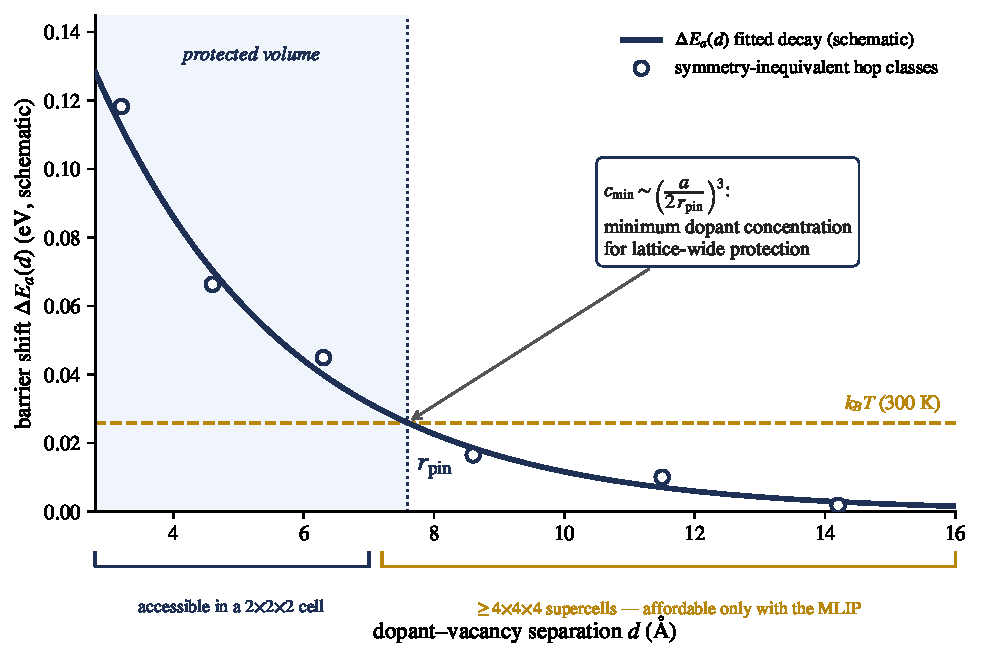
\includegraphics[width=0.86\textwidth]{figs/fig_pinning_radius.pdf}
\caption{Definition of the pinning radius (schematic). $\Delta E_a$ is computed for
symmetry-inequivalent hop classes at increasing dopant--vacancy separation $d$; the
fitted decay crosses the thermal scale $k_BT$ at $r_{\mathrm{pin}}$, the radius of the
protected volume. The decay tail lies beyond the reach of ranking-scale
$2\times2\times2$ cells and is accessible only with the MLIP; $r_{\mathrm{pin}}$
converts directly into the minimum dopant concentration for lattice-wide protection,
connecting cell-scale simulations to the trace doping levels used experimentally.}
\label{fig:pinning}
\end{figure}

% ================= 4 THEORY =================
\section{Theoretical Framework}

The methodology rests on five theory layers, each of which repairs the deficiency of
the layer above it.

\subsection{Layer 1: Born--Oppenheimer potential energy surface}
The mass separation between nuclei and electrons permits integration over electronic
degrees of freedom, defining a potential energy surface (PES)
$E(\mathbf{R}_1,\dots,\mathbf{R}_N)$ on which stable configurations are local minima,
migration transition states are first-order saddle points (Hessian with exactly one
negative eigenvalue), and $E_a = E_{\mathrm{saddle}} - E_{\mathrm{minimum}}$ along the
minimum-energy path (MEP). In this language, a pinning dopant is precisely a local
reshaping of the PES: deepening the valley or raising the pass.

\subsection{Layer 2: Harmonic transition-state theory}
Assuming Boltzmann equilibrium in the reactant basin, a dividing surface at the saddle,
and no recrossing, the hop rate takes the Vineyard form
\begin{equation}
\Gamma \;=\; \frac{\prod_{i=1}^{3N}\nu_i^{\mathrm{min}}}
{\prod_{i=1}^{3N-1}\nu_i^{\mathrm{saddle}}}
\exp\!\left(-\frac{E_a}{k_B T}\right),
\end{equation}
in which the prefactor varies by a factor of 2--3 across chemically similar dopants
while the exponential varies by orders of magnitude. This licenses a screening strategy
that ranks candidates by $E_a$ alone. The harmonic approximation is justified here
since $E_a/k_BT\approx20$ (deep-well limit), and quantum tunnelling is negligible for
an ion as heavy as iodide.

Halide perovskites are, however, strongly anharmonic, with double-well zone-boundary
phonons and pronounced dynamic disorder; static 0~K barriers and 300~K effective
barriers can therefore differ through entropic and prefactor contributions
(Meyer--Neldel compensation). Two safeguards address this. First, the screening
observable is the \emph{difference} $\Delta E_a$ between doped and undoped lattices, in
which anharmonic and entropic corrections cancel to first order --- the ranking is
more robust than any absolute barrier. Second, for the top-ranked candidates the
harmonic-TST picture is cross-checked by transition-state-theory-free molecular
dynamics (Section~5.3). In the FA-rich production host a third safeguard applies:
orientational disorder makes $E_a$ itself a distribution, so every FA-host barrier is
reported as an ensemble statistic (mean $\pm$ spread over MD-sampled FA orientations
and Cs placements) --- a protocol forced by our own preliminary finding that a
single-configuration GA$^+$ barrier shift varies by over 200~meV with cation
orientation (Section~6).

\subsection{Layer 3: Saddle-point location by CI-NEB}
The climbing-image nudged elastic band method (Henkelman, Uberuaga and J\'onsson, 2000)
discretises the path between two minima into images coupled by virtual springs, with
force projection --- spring forces retained only parallel to the path, true forces only
perpendicular --- preventing corner-cutting and image sliding. The highest-energy image
then climbs against the parallel component of the true force to converge exactly onto
the saddle point. CI-NEB (rather than plain NEB) is mandatory for quantitative $E_a$.

\subsection{Layer 4: DFT reference energies}
Kohn--Sham DFT provides the ground-truth PES at $\mathcal{O}(N^3)$ cost. Two lattices
divide the labour. Method development and the literature anchors use the fully
inorganic room-temperature $\gamma$-phase of CsPbI$_3$ (consistent with Arber et al.,
2025), whose broken symmetry is handled by explicit enumeration of inequivalent hop
directions and which decouples methodology from organic-cation degrees of freedom.
Production screening uses pseudo-cubic FA$_{0.95}$Cs$_{0.05}$PbI$_3$ supercells with
FA orientations drawn from thermalised MLIP-MD snapshots; dispersion correction (D3)
is mandatory once organic cations are present. Four system-specific corrections are
essential: (i) spin--orbit coupling for Pb is included in electronic-structure checks,
while migration barriers --- governed chiefly by ionic electrostatics and bond strength
--- are computed at the PBE(+D3) level after explicit SOC-sensitivity tests; (ii) the
dominant migrating defect is the positively charged iodide vacancy
$V_{\mathrm{I}}^{+}$, requiring finite-size electrostatic corrections of the
Freysoldt--Neugebauer--Van de Walle type (Freysoldt et al., 2009), the neglect of which
explains $\sim$0.1~eV discrepancies between literature values; because FNV is derived
for equilibrium point defects, its path-dependence along the MEP is monitored through
supercell-size tests; (iii) supercell convergence ($\geq2\times2\times2$, $\sim$96
atoms for the ranking campaign, with extrapolation tests) controls spurious
image--image interactions; (iv) PBE self-interaction error can artificially delocalise
charge around charged defects, so the top-three candidates receive HSE(+SOC)
single-point spot checks --- whose density of states doubles as the
electronic-benignity screen of Objective 3, one calculation serving two gates ---
before experimental hand-off.

\subsection{Layer 5: MLIP acceleration with active learning}
A single CI-NEB ($\sim$7 images $\times$ $\sim$100 ionic steps) costs thousands of
core-hours at the DFT level; the screening campaign requires $\sim$2000 such paths,
which is infeasible. The MACE equivariant message-passing architecture (Batatia et
al., 2022), via foundation models pre-trained on $\sim$$10^6$ Materials Project
configurations (Batatia et al., 2024), reduces force-evaluation cost by four orders of
magnitude. Its built-in $E(3)$-equivariance guarantees exact rotational behaviour of
energies and forces by construction, and message passing extends the effective
receptive field beyond the local cutoff. The starting checkpoint will be selected among
MACE-MP-0, MACE-MPA-0 and OMat24-trained models (Barroso-Luque et al., 2024) by
validation against the migration-barrier benchmark of Bheemaguli, Xiao and Sai Gautam
(2025), which identifies MACE-family models as the most accurate foundation MLIPs for
NEB barriers. Zero-shot \emph{absolute} barriers nonetheless carry errors of order
0.1~eV whose sign is system-dependent: PES softening biases many benchmarks low (Deng
et al., 2025), whereas our own DFT calibration on the CsPbI$_3$ $V_{\mathrm{I}}$ hop
finds a 1.84$\times$ \emph{overestimate} against PBE at fixed geometry, with the
saddle position and mechanism exactly reproduced (Section~6). Both observations point
the same way: zero-shot output seeds paths and identifies mechanisms; it never ranks.

\begin{riskbox}
\textbf{The central methodological risk --- and its remedy.} Foundation MLIPs are
trained predominantly on near-equilibrium configurations, whereas saddle points are
far-from-equilibrium structures lying precisely in the model's extrapolation regime ---
with absolute errors of order 0.1~eV in a system-dependent direction (measured at
1.84$\times$ high on this system; Section~6).
Zero-shot barriers are therefore never ranked: they serve only as \emph{path seeding},
a role in which foundation-model images outperform conventional interpolation in
$>$71\% of NEB setups (Bheemaguli et al., 2025). The remedy is a Bayesian
active-learning loop: committee-variance uncertainty flags the configurations the model
does not know (saddle-point regions are flagged almost by construction); DFT single
points are computed only there; the model is fine-tuned; the loop repeats until the
validation error satisfies
$|E_a^{\mathrm{MLIP}} - E_a^{\mathrm{DFT}}| < 0.03$--$0.05$~eV. Each expensive DFT call
is thereby spent where its information gain is maximal.
\end{riskbox}

\begin{keybox}
\textbf{Charge-state representation in the MLIP.} Standard MACE architectures are
charge-agnostic: the network sees only species and coordinates, so a foundation model
trained on charge-neutral cells effectively describes $V_{\mathrm{I}}^{0}$, not
$V_{\mathrm{I}}^{+}$ --- and these differ in mobility by an order of magnitude (Tyagi
et al., 2025). Every ranked $\Delta E_a$ is therefore computed with a model fine-tuned
\emph{exclusively} on charged-supercell DFT data at fixed composition and charge ---
one model per charge state, following the validated protocol of Tyagi et al.\ (2025).
Long-range electrostatic truncation error is monitored through supercell-size tests;
should it prove limiting, a latent-Ewald long-range layer compatible with MACE (Cheng,
2025) will be added, with multi-fidelity charged-defect schemes (Wang, Mosquera-Lois
and Walsh, 2026) as a further fallback.
\end{keybox}

% ================= 5 METHODOLOGY =================
\section{Methodology and Work Plan}

\subsection{Pipeline architecture}
Figure~\ref{fig:pipeline} summarises the six-phase pipeline and the division of labour
between the MLIP and the bounded DFT budget.

\begin{figure}[t]
\centering
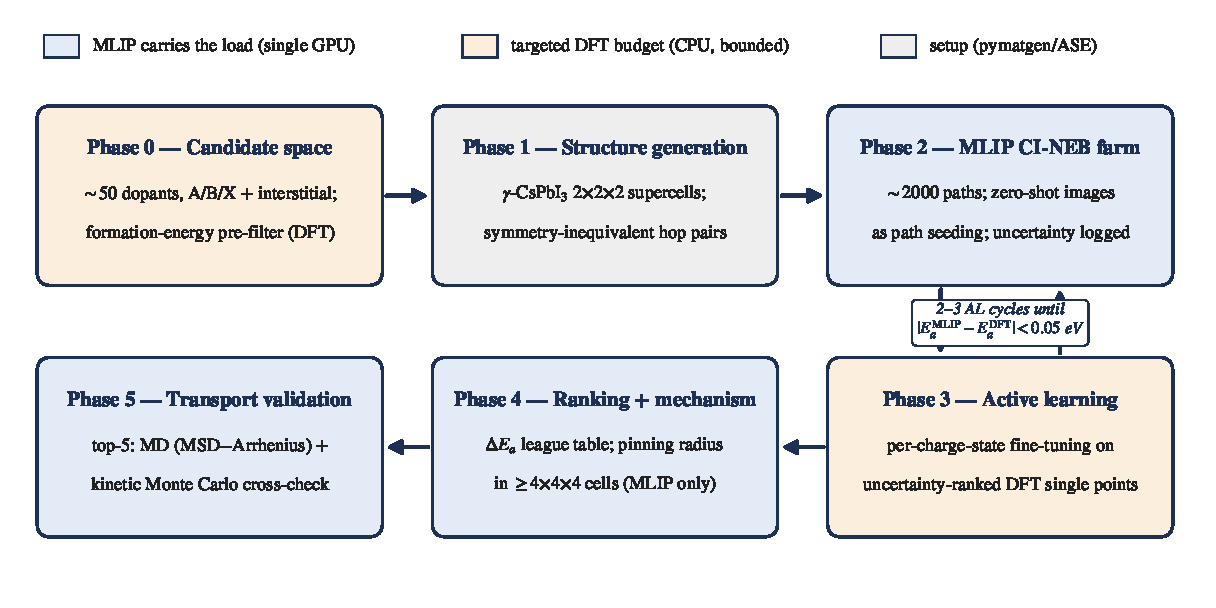
\includegraphics[width=\textwidth]{figs/fig_pipeline.pdf}
\caption{Screening pipeline. The MLIP (single GPU) carries $>$95\% of force
evaluations; the DFT budget (CPU) is front-loaded into validation anchors and targeted
by active-learning uncertainty. Zero-shot foundation-model output is used only to seed
migration paths; all ranked barriers come from per-charge-state fine-tuned models.}
\label{fig:pipeline}
\end{figure}

\begin{enumerate}[leftmargin=1.6em]
\item \textbf{Phase 0 --- Candidate space definition.} Assemble $\sim$50 dopants
across the four structural classes of Objective~2; pre-filter by computed dopant
formation energy to exclude synthetically implausible candidates.

\item \textbf{Phase 1 --- Structure generation} (pymatgen/ASE). Substitutional and
interstitial injection into FA$_{0.95}$Cs$_{0.05}$PbI$_3$ $2\times2\times5$
production cells (20 A-sites $\Rightarrow$ one Cs at exactly 5\%; FA orientations
from thermalised MLIP-MD snapshots) and $\gamma$-CsPbI$_3$ $2\times2\times2$
pre-screen cells; symmetry-inequivalent configuration enumeration; generation of
iodide-vacancy hop ensembles binned by dopant--vacancy distance (first shell, second
shell, remote bulk reference).

\item \textbf{Phase 2 --- MLIP relaxation and CI-NEB farm} (ASE + MACE). Foundation-model
IDPP-refined seeding of seven images; FIRE optimisation to
$f_{\mathrm{max}} < 0.03$~eV\,\AA$^{-1}$; per-path uncertainty logging.

\item \textbf{Phase 3 --- Active-learning closure} (2--3 cycles). Uncertainty-ranked
\emph{charged-supercell} DFT single points (VASP/Quantum ESPRESSO); training sets mixed
across endpoints, intermediate images, and perturbed configurations to prevent
saddle-point overfitting; per-charge-state fine-tuning; re-run. The ranked pre-screen
of Phase 4 uses fine-tuned models only.

\item \textbf{Phase 4 --- Ranking and mechanistic attribution.} $\Delta E_a$ league
table from the fine-tuned models; pinning-radius curves
$\Delta E_a(d_{\mathrm{dopant\text{--}vacancy}})$ extracted in $\geq4\times4\times4$
supercells; saddle-point fingerprints (bond lengths, hydrogen-bond counts, Bader
charges) mapped onto the three mechanism classes; an HSE-level density-of-states check
flags dopant-induced gap states, so the final table ranks candidates that pin the
lattice \emph{without} poisoning the optoelectronics.

\item \textbf{Phase 5 --- From barriers to transport.} For the top five candidates,
MLIP molecular dynamics ($\geq$10~ns, mean-square-displacement Arrhenius analysis)
provides a TST-free cross-check of $\Delta E_a$, benchmarked against the $\sim$80~ns
MD standard set by Arber et al.\ (2025); kinetic Monte Carlo over the computed rate
catalogue then yields macroscopic diffusion coefficients from two independent routes.
\end{enumerate}

\subsection{Twelve-month timeline}
\begin{table}[H]
\centering\small
\begin{tabular}{@{}p{1.6cm}p{8.3cm}p{4.6cm}@{}}
\toprule
\textbf{Months} & \textbf{Activity} & \textbf{Milestone} \\
\midrule
1--2 & Minimal viable pipeline: undoped $\gamma$-CsPbI$_3$, single $V_{\mathrm{I}}$
CI-NEB, zero-shot path seeding, DFT convergence and charged-defect correction budget &
Pipeline runs end-to-end; $E_a$ within literature range \\
3--4 & Objective 1 completion: relaxed charged paths (anchor b); FA-host bring-up
($\alpha$-FAPbI$_3$ + $2\times2\times5$ cells, orientational-ensemble protocol);
GA$^+$ natively in FA & Four anchors closed; FA baseline distribution \\
5--7 & Phases 1--2 at scale in the FA$_{0.95}$Cs$_{0.05}$ host (ensemble protocol);
CsPbI$_3$ pre-screen funnel; MLIP-NEB farm ($\sim$2000 paths) with first-cycle
fine-tuned models & Fine-tuned $\Delta E_a$ pre-screen \\
8--9 & Phase 3: active-learning closure; per-charge-state model validation &
$|E_a^{\mathrm{MLIP}}-E_a^{\mathrm{DFT}}|<0.05$~eV \\
10--11 & Phase 4: final ranking, pinning radii in large supercells, mechanism
fingerprints; Phase 5 for top five & Mechanism-annotated league table \\
12 & Write-up; code release and documentation & Dissertation + open-source repository \\
\bottomrule
\end{tabular}
\caption{Work plan. The DFT budget is concentrated in months 1--4 and 8--9; the
screening burden (months 5--7) is carried almost entirely by the MLIP.}
\end{table}

\subsection{Validation strategy}
Every layer carries an internal check: supercell-size extrapolation (Layer 4),
SOC-sensitivity tests on representative barriers (Layer 4), HSE spot checks on
top-ranked candidates (Layer 4), MLIP-vs-DFT barrier validation on a held-out path set
(Layer 5), TST-free MD cross-validation of the top five candidates (Phase 5), and, at
the physics level, the four anchors of Objective 1 --- three experimental, one
computational. No new-dopant prediction is reported unless all anchors are reproduced.

% ================= 6 PRELIMINARY RESULTS =================
\section{Preliminary Results}

The pipeline of Section~5 is not a plan on paper: it is running. In July 2026 the
MLIP leg (single RTX 5090) and the DFT leg (32-core Slurm nodes, Quantum ESPRESSO
7.5) were commissioned, and every result below is version-controlled with raw data
and one-command reproduction scripts in the project repository.

\begin{enumerate}[leftmargin=1.6em]
\item \textbf{Regression baseline.} $\gamma$-CsPbI$_3$ (159-atom $2\times2\times2$)
$V_{\mathrm{I}}$ edge hop: $E_a = 0.259$~eV forward / 0.230~eV reverse (zero-shot
MACE-MP-0, float64 CI-NEB), reproduced across CPU/GPU platforms and float32/64 to
$<0.1$~meV, and size-converged ($3\times3\times3$ agrees to 1~meV). This path is the
permanent cross-platform regression test for every future environment change.

\item \textbf{DFT calibration of the foundation model.} PBE single points on the
identical NEB geometries give a 141~meV barrier versus MACE's 259~meV --- a
1.84$\times$ overestimate with the saddle position and mechanism exactly reproduced.
This quantifies the zero-shot failure mode that Layer 5 anticipates and measures the
fine-tuning requirement rather than assuming it. The charged-cell DFT machinery also
runs end-to-end (fixed-geometry $V_{\mathrm{I}}^{+}$ barrier 127~meV vs
$V_{\mathrm{I}}^{0}$ 141~meV; relaxed charged paths are the immediate next step
toward the Tyagi-scale separation, which is a structural-relaxation effect).

\item \textbf{Strain anchor reproduced.} Biaxial strain from $-3\%$ to $+3\%$:
tensile lowers, compressive raises, slope $dE_a/d\varepsilon = -2.25$~eV per unit
strain ($r=-0.98$), and the strain response is finite-size robust (identical
$\Delta E_a$ at $2\times2\times2$ and $3\times3\times3$).

\item \textbf{GA$^+$ anchor: sign robust, magnitude ensemble-dependent.} All three
near-site cation orientations pin ($+70$ to $+278$~meV); a 16~\AA{} far-site control
gives $\approx 0$ --- the signature of a genuinely local mechanism, with
N--H$\cdots$I saddle contacts of 2.4--2.7~\AA{} supporting the hydrogen-bond-anchoring
picture. The magnitude, however, converges in neither orientation (207~meV spread)
nor cell size ($+70 \to +335$~meV at $3\times3\times3$): the empirical finding that
forces the ensemble-and-large-cell protocol now built into Objectives 2--3.

\item \textbf{Five-dopant zero-shot screen with mechanism labels.} Every first-shell
substitutional candidate tested (Sr$^{2+}$, Ca$^{2+}$, Ba$^{2+}$, Bi$^{3+}$ on Pb;
Br$^-$ on I) \emph{lowers} the barrier --- an honest negative result independently
consistent with the B-site null result of Arber et al.\ (2025), with saddle-geometry
fingerprints separating direct edge-contact from remote bond-modulation mechanisms,
and a first pinning-radius curve (Sr: perturbation radius $\approx 5$~\AA). This
redirects screening priority toward interstitial and channel-blocking chemistries,
exactly as Section 2.1(4) anticipated.

\item \textbf{Measured throughput.} $\sim$1500 CI-NEB paths/hour on one GPU (after
per-image-calculator and batching fixes) and $\approx$33~min per 159-atom DFT single
point on 32 cores: the Phase-2 farm size and the DFT budget of Section~5 are measured
quantities, not estimates.
\end{enumerate}

% ================= 7 RISK =================
\section{Risk Assessment}

Table~2 ranks the principal risks by severity. Both High-severity risks carry
\emph{structural} mitigations already embedded in the pipeline design --- restriction
of zero-shot output to path seeding, and per-charge-state fine-tuning --- rather than
contingencies bolted on after the fact.

\begin{table}[H]
\centering\small
\begin{tabular}{@{}p{4.6cm}p{1.5cm}p{8.2cm}@{}}
\toprule
\textbf{Risk} & \textbf{Severity} & \textbf{Mitigation} \\
\midrule
MLIP extrapolation failure at saddle points & High & Zero-shot output restricted to
path seeding; active learning with uncertainty sampling; mandatory DFT spot checks on
all top-ranked candidates \\
Charge-state misrepresentation in the MLIP & High & Per-charge-state fine-tuning on
charged-supercell data (Tyagi et al., 2025); FNV corrections throughout; benchmark
against published $V_{\mathrm{I}}$ values \\
Long-range electrostatics beyond MLIP cutoff & Medium & Supercell-size monitoring;
latent-Ewald augmentation (Cheng, 2025) or multi-fidelity schemes (Wang et al., 2026)
as fallback \\
Bulk-only scope vs GB-dominated transport in films & Medium & Bulk $\Delta E_a$ sets
the intrinsic floor for hysteresis and drift; grain-boundary supercells are a natural
pipeline extension (Pols et al., 2024) \\
Organic-cation orientational sampling & Medium & Method development on CsPbI$_3$;
orientation-averaged barriers for hybrid compositions \\
Finite-size effects & Medium & Supercell convergence tests with extrapolation;
two-tier small/large-cell design \\
Single-hop picture misses collective effects & Medium & Phase 5 kMC/MD
cross-validation \\
Candidate dopants synthetically inaccessible & Medium & Formation-energy pre-filter in
Phase 0 \\
Migration-optimal dopant degrades optoelectronic performance & Medium & HSE
density-of-states benignity gate in Phase 4 (band edges are Pb--I-derived, so A-site
and interstitial dopants are low-risk a priori); pinning radius minimises the required
concentration \\
Composition transferability (CsPbI$_3$ pre-screen $\to$ FA-rich host) & Medium &
Two-tier funnel with the rank correlation reported as an explicit deliverable;
anchors re-established per host; GA anchor computed natively in the FA lattice \\
FA orientational disorder inflates per-dopant cost ($\sim$10--30$\times$) & Medium &
Ensemble sizes set by the measured orientation spread; 1500 paths/hr farm absorbs
the multiplier; distributions, not single numbers, are the deliverable \\
HPC allocation shortfall & Low & MLIP carries $>$95\% of force evaluations; DFT budget
is bounded and front-loaded \\
\bottomrule
\end{tabular}
\caption{Principal risks and mitigations.}
\end{table}

% ================= 7 OUTCOMES =================
\section{Expected Outcomes and Impact}

\begin{enumerate}[leftmargin=1.6em]
\item \textbf{A mechanism-annotated dopant ranking} --- the first systematic
$\Delta E_a$ league table at the $\sim$50-candidate scale in which every entry carries
a saddle-point-resolved mechanistic label, directly answering the field's acknowledged
inability to specify which defect species each strategy immobilises.

\item \textbf{The pinning radius as a new design metric} --- the decay length of
$\Delta E_a$ with dopant--vacancy separation determines the minimum dopant
concentration for lattice-wide protection,
$c_{\min}\sim (a/2r_{\mathrm{pin}})^{3}$, a quantity inaccessible to experiment but
decisive for formulation, and the quantitative bridge between simulation-cell dopant
fractions and experimental trace-doping levels. Because every adverse electronic side
effect of doping --- bandgap shift, band tailing, secondary phases --- grows
monotonically with concentration, $r_{\mathrm{pin}}$ is simultaneously the
performance-preservation metric: the best dopant protects the lattice at the lowest
electronic cost.

\item \textbf{Transferable open infrastructure} --- the released pipeline generalises
immediately to bromide and mixed-halide systems, tin-based perovskites, grain-boundary
supercells, and, beyond photovoltaics, to any vacancy-mediated transport problem
(solid electrolytes, memristors).

\item \textbf{Experimental hand-off} --- the top three to five candidates constitute
concrete, falsifiable synthesis targets for collaborating device laboratories, with
temperature-dependent conductivity as the direct experimental test of the predicted
$\Delta E_a$; every handed-off candidate is certified both kinetically (HSE-verified
barrier) and electronically (no dopant-induced gap states).
\end{enumerate}

% ================= 8 FEASIBILITY =================
\section{Feasibility}

The candidate brings (i) hands-on device-fabrication context from a p--i--n perovskite
fabrication and characterisation programme (HTL/SAM, perovskite, ETL and electrode
deposition; XRD, SEM, $J$--$V$/EQE and maximum-power-point stability measurement),
grounding the computational choices in device reality --- notably the buried-interface
strain relevance of the SAM layer; (ii) prior experience with the exact
machine-learning methodology required, including graph-neural-network training with
active-learning cycles (validation MAE 0.067~ppm in an NMR chemical-shift project) and
Bayesian-optimisation experiment design; and (iii) working familiarity with the
ASE/pymatgen/MACE software stack. The project is further de-risked by design: the
months 1--4 milestones deliberately reproduce published results (Eames et al., 2015;
Tyagi et al., 2025), so the novel screening campaign launches from a validated
baseline rather than an untested pipeline. Compute requirements are modest: the MLIP
carries the screening load on a single GPU, while the bounded DFT budget ($\sim$$10^2$
single-point batches plus $\sim$20 full NEB benchmarks) fits within a standard
university HPC allocation.

% ================= REFERENCES =================
\section*{References}
\addcontentsline{toc}{section}{References}
\begin{list}{}{\setlength{\itemindent}{-1.2em}\setlength{\leftmargin}{1.2em}\setlength{\itemsep}{0.25em}\small}

\item Arber, A.N., Mocanu, F.C. and Islam, M.S. (2025) `Ion migration and dopant
effects in the gamma-CsPbI$_3$ perovskite photovoltaic material: atomistic insights
through ab initio and machine learning methods', \emph{Chemistry of Materials}, 37.
doi: 10.1021/acs.chemmater.5c00503

\item Barroso-Luque, L. et al. (2024) `Open Materials 2024 (OMat24) inorganic
materials dataset and models', \emph{arXiv preprint}, arXiv:2410.12771.

\item Batatia, I., Kov\'acs, D.P., Simm, G.N.C., Ortner, C. and Cs\'anyi, G. (2022)
`MACE: higher order equivariant message passing neural networks for fast and accurate
force fields', \emph{Advances in Neural Information Processing Systems}, 35,
pp. 11423--11436.

\item Batatia, I. et al. (2024) `A foundation model for atomistic materials
chemistry', \emph{arXiv preprint}, arXiv:2401.00096.

\item Bheemaguli, A.K., Xiao, P. and Sai Gautam, G. (2025) `Evaluation of foundational
machine learned interatomic potentials for migration barrier predictions',
\emph{arXiv preprint}, arXiv:2512.03642.

\item Cheng, B. (2025) `Latent Ewald summation for machine learning of long-range
interactions', \emph{npj Computational Materials}, 11, 80. doi:
10.1038/s41524-025-01577-7

\item Deng, B., Choi, Y., Zhong, P. et al. (2025) `Systematic softening in universal
machine learning interatomic potentials', \emph{npj Computational Materials}, 11, 9.
doi: 10.1038/s41524-024-01500-6

\item Du, N. et al. (2026) `Taming lattice strain via buried interface engineering for
reverse-bias resilient perovskite solar cells', \emph{Nano-Micro Letters}, 18, 387.
doi: 10.1007/s40820-026-02244-2

\item Eames, C., Frost, J.M., Barnes, P.R.F., O'Regan, B.C., Walsh, A. and Islam, M.S.
(2015) `Ionic transport in hybrid lead iodide perovskite solar cells', \emph{Nature
Communications}, 6, 7497. doi: 10.1038/ncomms8497

\item Freysoldt, C., Neugebauer, J. and Van de Walle, C.G. (2009) `Fully ab initio
finite-size corrections for charged-defect supercell calculations', \emph{Physical
Review Letters}, 102(1), 016402. doi: 10.1103/PhysRevLett.102.016402

\item Henkelman, G., Uberuaga, B.P. and J\'onsson, H. (2000) `A climbing image nudged
elastic band method for finding saddle points and minimum energy paths', \emph{Journal
of Chemical Physics}, 113(22), pp. 9901--9904. doi: 10.1063/1.1329672

\item Lee, J.-W., Tan, S., Seok, S.I., Yang, Y. and Park, N.-G. (2022) `Rethinking the
A cation in halide perovskites', \emph{Science}, 375(6583), eabj1186. doi:
10.1126/science.abj1186

\item Li, Z. et al. (2022) `Inhibiting ion migration by guanidinium cation doping for
efficient perovskite solar cells with enhanced operational stability', \emph{Solar
RRL}, 6, 2200003. doi: 10.1002/solr.202200003

\item Liu, D. et al. (2021) `Strain analysis and engineering in halide perovskite
photovoltaics', \emph{Nature Materials}, 20, pp. 1337--1346. doi:
10.1038/s41563-021-01097-x

\item Muscarella, L.A. and Ehrler, B. (2022) `The influence of strain on phase
stability in mixed-halide perovskites', \emph{Joule}, 6(9), pp. 2016--2031. doi:
10.1016/j.joule.2022.07.005

\item Muscarella, L.A. et al. (2020) `Lattice compression increases the activation
barrier for phase segregation in mixed-halide perovskites', \emph{ACS Energy Letters},
5(10), pp. 3152--3158. doi: 10.1021/acsenergylett.0c01474

\item Pols, M. et al. (2024) `Ion migration at metal halide perovskite grain
boundaries elucidated with a machine learning force field', \emph{Journal of Physical
Chemistry Letters}, 15(50), pp. 12362--12369. doi: 10.1021/acs.jpclett.4c03332

\item Thiesbrummel, J., Mili\'c, J.V., Deibel, C., Garnett, E.C., Tao, S., Kirchartz,
T., Guerrero, A., Cameron, P., Tress, W., Islam, M.S. and Ehrler, B. (2026) `Ion
migration in perovskite solar cells', \emph{Nature Reviews Chemistry}. doi:
10.1038/s41570-025-00790-8

\item Tyagi, V., Pols, M., Brocks, G. and Tao, S. (2025) `Tracing ion migration in
halide perovskites with machine learned force fields', \emph{Journal of Physical
Chemistry Letters}, 16(20), pp. 5153--5159. doi: 10.1021/acs.jpclett.5c01139

\item Vineyard, G.H. (1957) `Frequency factors and isotope effects in solid state rate
processes', \emph{Journal of Physics and Chemistry of Solids}, 3(1--2), pp. 121--127.
doi: 10.1016/0022-3697(57)90059-8

\item Wang, X., Mosquera-Lois, I. and Walsh, A. (2026) `Multi-fidelity machine
learning interatomic potentials for charged point defects', \emph{arXiv preprint},
arXiv:2603.05238.

\item Xue, D.-J. et al. (2020) `Regulating strain in perovskite thin films through
charge-transport layers', \emph{Nature Communications}, 11, 1514. doi:
10.1038/s41467-020-15338-1

\item Zhao, Y. et al. (2022) `Suppressing ion migration in metal halide perovskite via
interstitial doping with a trace amount of multivalent cations', \emph{Nature
Materials}, 21, pp. 1396--1402. doi: 10.1038/s41563-022-01390-3

\end{list}

\end{document}
